\documentclass[xcolor=dvipsnames]{beamer}

\usepackage{amssymb,amsmath}
%\usepackage[T2A,T1]{fontenc}
\usepackage[utf8]{inputenc}
\usepackage[russian]{babel}
\usepackage{amsthm}
\usepackage{amsfonts}
\usepackage{algorithmic, algorithm}
\usepackage{xcolor}
\usepackage{graphicx}
\graphicspath{ {images/} }

%\usepackage{cmap}
%\usepackage{lmodern}
\newtheorem*{mynote}{Замечание}
\newtheorem{mydef}{Определение}
\newtheorem{mytheorem}{Теорема}
\newtheorem{statement}{Утверждение}
\newtheorem*{consequence}{Следствие}

\def \eval #1#2{\left.#1\right\vert_{#2}}
\def \<#1> {\langle #1 \rangle}
\def \n #1{\mathit{#1}}
\def \bigcupn {\bigcup\limits_{v=1}^{n}}
%Information to be included in the title page:
\title{Использование логических формул для кэширования универсальных запросов к Реляционной Базе Данных.}
\author{Мосин С.В.}
\institute{ИМ СО РАН (ОмФ)}
\date{2015}

\usetheme{Boadilla}
%\usecolortheme{seahorse}
\usefonttheme{serif}
%[onlymath]
%\usefonttheme{structuresmallcapsserif}
%\usepackage{mathptmx}
%\usepackage{mathptmx}
%\usepackage[scaled=0.9]{helvet}
%\usepackage{courier}

\setbeameroption{show notes}

\setbeamertemplate{note page}[plain]
\setbeamertemplate{theorems}[numbered]
\setbeamertemplate{footline}{%
    \raisebox{5pt}{\makebox[\paperwidth]{\hfill\makebox[20pt]{\color{gray}
          \scriptsize\insertframenumber}}}\hspace*{5pt}}
          
%\setbeamercolor*{frametitle}{bg=white, fg=brown}

\begin{document}
 
\frame{\titlepage}
 
\begin{frame}
\frametitle{Содержание}
\tableofcontents
\end{frame}


\section{Клиент-серверная архитектура}

\begin{frame}
\frametitle{\insertsection}
\begin{center}
  \makebox[\textwidth]{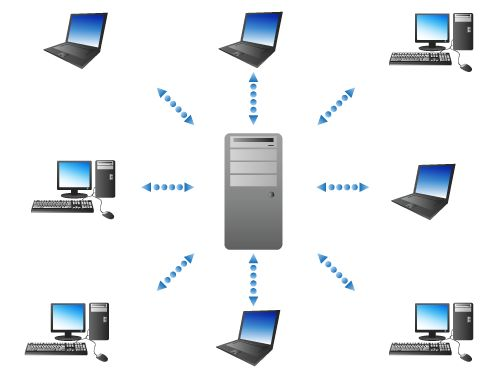
\includegraphics[width=0.6\paperwidth]{client-server}}
\end{center}
\end{frame}
\note{В данной работе рассматривается новый метод кэширования запросов к реляционной базе данных для систем с центральным сервером и распределенными клиентами. Данные загружаются в клиентский кэш, основываясь на запросах, выполненных на сервере БД.}


\begin{frame}
\frametitle{Обзор существующих работ}
\begin{itemize}
 \item<1->S.~Zykin, A.~Poluyanov, Multidimensional data building using intermediate
   representations., Administration problems~(5) (2013) 54--59.
 \item<2-> C.-S. Park, M.-H. Kim, Y.-J. Lee, Usability-based caching of query results in
   olap systems., Journal of Systems and Software 68~(2) (2003) 103--119.
 \item<2-> E.~Baralis, S.~Paraboschi, E.~Teniente,
   \href{http://dl.acm.org/citation.cfm?id=645923.671019}{Materialized views
   selection in a multidimensional database}, in: Proceedings of the 23rd
   International Conference on Very Large Data Bases, VLDB '97, Morgan Kaufmann
   Publishers Inc., San Francisco, CA, USA, 1997, pp. 156--165.
 \item<2->  P.~Kalnis, D.~Papadias, Proxy-server architectures for olap., in: S.~Mehrotra,
    T.~K. Sellis (Eds.), SIGMOD Conference, ACM, 2001, pp. 367--378.
\end{itemize}
\note<1>{Данная работа основывается на результатах, полученных в
статье Сергея Владимировича Зыкина и Андрея Полуянова. Устранено условие, ограничивающее атрибуты
промежуточного представления, а также сделано обобщение теорем на случай нескольких
промежуточных представлений.}
\note<2>{Множество публикаций посвящено проблеме управления содержимым кэша.

В первой работе эвристические алгоритмы обновляют кэш, основываясь на данных пользователя
и динамически подстраиваясь под них.

В следующей статье предлагается статический выбор наиболее важных пользовательских запросов
с последующим применением статистических алгоритмов для дополнения кэша

В последней статье исследуется хранение кэшированных данных на различных удаленных серверах.

Наша статья решает проблему наилучшего использования имеющегося кэша для исполнения
пользовательских запросов. Управление кэшем и наилучшее использование кэша - это две
взаимодополняющие задачи.}
\end{frame}
 %--------------------------------------------------------------------------------------- %
 
 
\section{Обзор существующих работ}

\begin{frame}
\frametitle{\insertsection}
\begin{itemize} 
 \item<1-> F.~N. Afrati, C.~Li, P.~Mitra, Rewriting queries using views in the presence of
    arithmetic comparisons., Theor. Comput. Sci. 368~(1-2) (2006) 88--123.
 \item<2-> A.~M. Keller, J.~Basu, A predicate-based caching scheme for client-server
    database architectures, VLDB J. 5~(1) (1996) 35--47.
 \item<3-> J.~Shim, P.~Scheuermann, R.~Vingralek, Dynamic caching of query results for
    decision support systems., in: SSDBM, 1999, pp. 254--263.
\end{itemize}
\note<1>{Наиболее близка к рассматриваемой проблеме работа Фото Афрати. В ней рассматриваются
конъюнктивные запросы над доменами данных с предикатами в виде арифметических сравнений и
представлены алгоритмы вычисления запросов с использованием существующих представлений.}
\note<2>{В следующей работе решается задача анализа содержимого кеша, при этом промежуточным
представлениям в кэше ставятся в соответствие предикаты. Проблема использования кэша
решается за счет выводимости предикатов. В данной работе эту проблему предлагается решать за счет
вычисления областей истинности формул соответствующих пользовательских запросов, результаты которых
находятся в кеше.}
\note<3>{Завершает список работ со схожей тематикой статья, в которой предпринята попытка решить
как задачу использования, так и управления кэшем. Кэш используется как при полном совпадении
запросов, так и в определенных условиях в случае если результаты кэша объемлют требуемый запрос.}
\end{frame}
 %---------------------------------------------------------------------------------------%


\section{Пример использования кэша}

\begin{frame}
\frametitle{\insertsection}
Рассмотрим фрагмент схемы БД, представляющий учебный план в универитете:
\vspace{\baselineskip}

$R_1 =\mbox{\it Студенты}\ (\mbox{\bf № студента}, \mbox{ФИО студента},
\mbox{Группа})$\\
$R_2 =\mbox{\it Расписание}\ (\mbox{\bf Группа}, \mbox{\bf № аудитории},
\mbox{Дисциплина})$\\
$R_3 =\mbox{\it Успеваемость}\ (\mbox{\bf № студента}, \mbox{\bf Дисциплина},
\mbox{Оценка})$
\note{На слайде фрагмент БД, где представлены 3 отношения. Имена отношений выделены курсивом, их
первичные ключи - жирным шрифтом.
Номер студента уникально определяет его имя и группу, у данной группы в конкретной аудитории
проходят занятия по данной конкретной дисциплине, а номер студента и дисциплина соответствуют одной
единственной оценке.}
\end{frame}


\begin{frame}
\frametitle{\insertsection}
\underline{Запрос 1}: Список студентов, изучающих физику, чей номер больше 210:
$$P_1 = \pi_{X_1}(\sigma_{F_1} (R_1 \Join R_2)),$$
где $\pi_{X_1}$ -- проекция по множеству атрибутов $X_1$
$X_1 = \{\text{№ студента},
\text{ФИО студента}, \text{Группа}, \text{Дисциплина}\}$,
$\sigma$ -- операция селекции,
$F_1$ -- логическая формула: $F_1 = (\text{№ студента} > 210\ \&\ \text{Дисциплина} =
\text{Физика})$, $\Join$ --операция естественного соедения.
\note{В результате данного запроса будут получены те кортежи БД, которые удовлетворяют формуле
$F_1$, причем с сервера будут запрошены только атрибуты $\text{№ студента},
\text{ФИО студента}, \text{Группа}, \text{Дисциплина}$}
\end{frame}


\begin{frame}
\frametitle{\insertsection}
\underline{Запрос 2}: Ведомости группы M10:
$$P_2 = \pi_{X_2}(\sigma_{F_2} (R_1 \Join R_3)),$$
где
$X_2 = \{\text{№ студента}, \text{Группа}, \text{Дисциплина}, \text{Оценка}\}$, $F_2$
-- логическая формула:\\
$F_2 = (\text{Группа}=\text{M10})$.
\note{Аналогично осуществляется Запрос 2, представляющий набор ведомостей по всем предметам для
студентов группы M10.}
\end{frame}


\begin{frame}
\frametitle{\insertsection}
$$P^{\ast} = \pi_{X^{\ast}}(\sigma_{F^{\ast}} (R_1 \Join R_2 \Join R_3 )),$$
где $X^{\ast}= \{\text{№ студента}, \text{Группа}, \text{Оценка}\}$, $F^{\ast}$
-- логическая формула: $F^{\ast} = (\textcolor<2>{blue}{\text{№ студента} > 300}\ \&\ 
\textcolor<3>{PineGreen}{\text{Группа} = \text{M10}}\ \&\ \textcolor<2>{brown}{\text{Дисциплина} = \text{Физика}})$.

\only<2>{$F_1 = (\textcolor{blue}{\text{№ студента} > 210}\ \&\ \textcolor{brown}{\text{Дисциплина} =
\text{Физика}})$}
\only<3>{$F_2 = (\textcolor{PineGreen}{\text{Группа}=\text{M10}})$.}

\vspace{\baselineskip}

Запрос может быть выполнен с использованием кэша:
$P^{\ast} =\pi_{X^{\ast}}(\sigma_{F_3} (P_1 \Join P_2 ))$, где $F_3$
-- логическая формула: $F_3 = (\text{Stud\_ID} > 300)$. 
\note<1>{Предположим теперь, что, пользователь хочет получить информацию, формализованную следующим
запросом (запрос $P^{\ast}$ на слайде)}
\note<2-3>{Сравнивая области истинности логических формул, используемых в $P_1$, $P_2$ и $P^{\ast}$,
получаем, что запрос может быть выполнен с помощью кэша.

Запрос к серверу в этом случае не требуется.}
\end{frame}
 %--------------------------------------------------------------------------------------- %


\section{Логические ограничения}

\begin{frame}
\frametitle{\insertsection}
Общий вид логической формулы:
\begin{equation}
F = K_1 \vee K_2 \vee \dots \vee K_m ,
\label{def_F_1}
\end{equation}
\begin{equation}
K_i = T_1 \&\ T_2 \dots \&\ T_n, i = 1, \dots, m ,
\label{def_F_2}
\end{equation}
здесь $T_j, j = 1, \dots, n$ - предикаты на множестве атрибутов БД

\begin{mynote}
Будем рассматривать расширенные имена атрибутов БД, где атрибут
$A_j$ в отношении $R_i$ носит название $R_i.A_j$.
\end{mynote}
\note{
Чтобы упростить вычисления областей истинности, будем рассматривать логические формулы в
Дизъюнктивной Нормальной Форме (ДНФ)

Замечание: Таким образом, можно избежать коллизий имен одинаковых атрибутов из разных отношений}

\begin{mydef}
Множество атрибутов, содержащихся в формуле, определяет её размерность и обозначается $\<F> $.

\begin{equation}
\<F> = \{R_1^F.A_1^F, \dots, R_k^F.A_k^F\} .
\label{def_F_3}
\end{equation}
\end{mydef}
\end{frame}


\begin{frame}
\frametitle{\insertsection}
\begin{itemize}
  \item<1-> операция сравнения $ \n{Expr}_1\ \theta\ \n{Expr}_2\ $, $\theta$ – операция
  сравнения $(\theta \in \{=, \neq, >, <, \leq, \geq\})$, $\n{Expr}_i$ –
  согласованные по типам допустимые выражения, определенные на множестве
  расширенных имен атрибутов и констант;
  \item<2-> операция $\n{Expr}_1\ \n{[NOT]}\ \n{BETWEEN}\ \n{Expr}_2\ \n{AND}\
  \n{Expr}_3$ (содержимое в прямоугольных скобках $[*]$ для предиката не
  является обязательным при написании);
  \item<3-> операция $\n{Expr}\ \n{[NOT]}\ \n{IN}\ S$, где $S$ – список значений либо
  подзапрос, результатом которого является столбец атрибута $A_j$ в отношении
  $R_i$;
  \item<4-> операция $\n{Str}_1\ \n{[NOT]}\ \n{LIKE}\ \n{Str}_2$, где $\n{Str}_i$ –
  строки;
  \item<5-> операция $\n{Expr}\ \theta\ \n{ALL/ANY}\ S$.
\end{itemize}
\note<1>{Обычное сравнение двух операторов, как пример, Группа = M10.}
\note<2>{Оператор (не) содержится в указанных границах.}
\note<3>{Оператор (не) содержится в списке значений. Отличие от предыдущей операции в том, что
здесь указывается полный перечень возможных значений атрибута, тогда как в $\text{BETWEEN}$ лишь
крайние значения.}
\note<4>{Оператор (не) подходит под указанный паттерн. Это специальное строковое сравнение с
использованием подобия регулярных выражений.}
\note<5>{Операция сравнения $\theta$ выполнена со всеми (ALL), хотя бы с одним из значений из списка (подзапроса) $S$

Перечисленные варианты операций используют не все возможности языка SQL. Например, предикат
$\n{EXISTS}$ не используется, поскольку в нем явно не специфицированы расширенные имена атрибутов,
предикат $\n{NULL}$ используется в данной работе для другой цели.}
\end{frame}


\begin{frame}
\frametitle{\insertsection}
$\forall R_i.A_j \in \<F> $:\\
<<Использование неопределенного значения>>: <<Да>> или <<Нет>>.\\
<<Нет>>: $\forall t$ - кортеж БД $t[R_i.A_j] = NULL \rightarrow t$ исключается из рассмотрения

\note{При вычислении логического выражения может быть получено значение UNKNOWN, если на текущем
кортеже t атрибут принимает значение NULL, поскольку результаты вычисления логических выражений в
SQL-запросах соответствуют трехзначной логике. Это приводит к неоднозначной интерпретации результата
не только обычными пользователями, но и опытными программистами.

Для решения этой проблемы предлагается ограничение: каждому атрибуту, входящему в $F^{\ast}$, явно
присваивается признак <<Использование неопределенного значения>> с двумя взаимоисключающими
значениями <<Да>> или <<Нет>>. Семантика этого признака такова, что если ему присвоено значение
<<Да>>, то появление значения $\n{NULL}$ для указанного атрибута в текущем кортеже $t$ не служит
основанием удаления этого кортежа из дальнейшего рассмотрения. В противном случае значение признака
<<Нет>> гарантирует, что появление значения $\n{NULL}$ для указанного атрибута в текущем кортеже $t$
приведет к удалению этого кортежа из дальнейшего рассмотрения.}
\end{frame}


\begin{frame}
\frametitle{\insertsection}
Запишем формулу (\ref{def_F_1}) для $F$ в следующем виде:

\vspace{\baselineskip}

$ F ( \dots, T_j , \dots )$,
где $T_j$ - предикаты формулы (\ref{def_F_2}).

\vspace{\baselineskip}

После преобразования:

\vspace{\baselineskip}

$F( \dots, T'_j , \dots )\wedge_{i,j}(R_i .A_j \neq  \n{NULL})$, где\\
\begin{itemize}
\item $\wedge_{i,j}(R_i .A_j \neq \n{NULL})$ - конъюнкция по всем атрибутам формулы $F$, для которых
не допустимо значение $\n{NULL}$.
\item Операция $T'_j = (T_j \vee_{i,j}(R_i .A_j = \n{NULL}))$, где  $\vee_{i,j}(R_i .A_j =
\n{NULL})$ - дизъюнкция по всем атрибутам предиката $T_j$, для которых допустимо значение
$\n{NULL}$.
\end{itemize}
\note{После проведения предложенного преобразования формула примет следующий вид.

Внешние скобки для предиката $T'_j$ определяют приоритет выполнения операций.

Несложно убедиться, что в рамках трехзначной логики преобразованная формула принимает только
значения $\n{TRUE}$ и $\n{FALSE}$. Кроме того, несложно убедиться, что в рамках двузначной логики,
когда в кортежах отсутствуют неопределенные значения, исходная формула $F$ будет эквивалентна
преобразованной формуле, поэтому семантика представления $P$ практически не искажается.

Здесь и далее будем считать все формулы F преобразованными}
\end{frame}


\begin{frame}
\frametitle{\insertsection}
$\mathcal{A} =$ $\{(a_1, \dots, a_n) \mid a_i \in Dom(A_i), i=1,\dots,n\}$, где $Dom(A_i)$ -
множество всех допустимых значений атрибута $A_i$.

\vspace{\baselineskip}

$\mathcal{A} = Dom(A_1)\times Dom(A_2)\times \dots \times Dom(A_n)$ - $n$-мерное пространство
значений всех атрибутов базы данных. Текущее состояние базы данных соответствует подмножеству этого
пространства.

\begin{block}{Пример}
\textcolor<2>{blue}{$\mathcal{A} = Dom(\text{№ студента})\times Dom(\text{ФИО студента}) \times
Dom(\text{Группа}) \times Dom(\text{№ аудитории}) \times Dom(\text{Дисциплина}) \times
Dom(\text{Оценка}) = $}
\textcolor<3->{blue}{$ \{205,315,461\} \times \{\text{Иван Иванов, Петр Петров, Василий Сидоров}\}
\times \{\text{M10, M11}\} \times \{100, 101, 102, 103\} \times \{\text{Физика, Химия}\} \times
\{3, 4, 5\} $}
\end{block}
\note<1>{Введем в рассмотрение множество $\mathcal{A}$.

Данное множество суть декартово произведение областей определения всех атрибутов, определенных в БД.

Допустимые состояния БД образуют лишь некоторую область в этом пространстве, соответствующую
ограничениям целостности на данные.}
\note<2>{Синим выделено декартово произведение всех атрибутов в БД из рассмотренного примера.}
\note<3>{Теперь выделение показывет возможные области определения атрибутов. Все их комбинации и
образуют множество $\mathcal{A}$.

Очевидно, что данное множество содержит больше данных, чем может быть состояний в БД. Например, в данном множестве содержатся точки, сопоставляющие
каждому из студентов каждый из номеров, тогда как у каждого студента такой номер уникален по ограничению
первичного ключа.}
\end{frame}


\begin{frame}
\frametitle{\insertsection}
\begin{mynote}
Размерность формулы $F$ может быть меньше
размерности $\mathcal{A}$, при этом атрибуты, не входящие в формулу, могут
принимать любые значения.
\end{mynote}

\begin{block}{Пример}
$F_1 = (\text{№ студента} > 210\ \&\ \text{Дисциплина} = \text{Физика}) \rightarrow \<F> = 2$.

\vspace{\baselineskip}

Эквивалентное представление:
\begin{multline*}
F_1 = (\text{№ студента} > 210\ \&\ \text{Дисциплина} = \text{Физика}\ \&\ \text{ФИО студента}\\
\textit{IN}\
\{\text{Иван Иванов, Петр Петров, Василий Сидоров}\}\ \&\ \text{Группа}\ \textit{IN}\\
\{\text{M10, M11}\} \&\ \text{№ аудитории}\ \textit{IN}\ \{100, 101, 102, 103\}\ \&\ \text{Оценка}\ \textit{IN}\\
\{70, 80, 90\})
\end{multline*}
\end{block}
\note{Если размерность формулы меньше размерности множества $\mathcal{A}$, то нами будет
рассматриваться эквивалентная формула $F$, у кототрой все отсутствующие атрибуты принимают любые
значения из своих доменов.

Рассмотрим преобразование одной из формул примера.

\textbf{\{пример\}}

Данное условие было введено для того, чтобы позволить сравнивать формулы различных размерностей}
\end{frame}


\begin{frame}
\frametitle{\insertsection}
\begin{mydef}
Областью истинности формулы $F$, опредененной (\ref{def_F_1}),
(\ref{def_F_2}), (\ref{def_F_3}), называется множество $M (F) = \{a \in \mathcal{A} \mid
F(a) = \n {TRUE}\}$.
\end{mydef}

\begin{block}{Пример}
$F_1 = (\text{№ студента} > 210\ \&\ \text{Дисциплина} = \text{Физика})$

\vspace{\baselineskip}

$M (F_1) = $ \{(315, Иван Иванов, M10, 100, Физика, 4), (315, Петр Петров, M10, 100, Физика, 4),
\dots (461, Василий Сидоров, M10, 100, Физика, 5)\}
\end{block}
\note{На данном слайде приведено понятие, на котором во многом основывается данная работа. Это
определение области истинности логической формулы.

На практике область истинности определяет все кортежи БД, которые удовлетворяют данной формуле, а
следовательно будут возвращены с сервера в ответ на пользовательский запрос. Однако обращаю внимание,
что в определении не используется конкретная реализация БД, а это значит, что области истинности
можно сравнивать аналитически, не осуществляя каких-либо запросов к серверу БД.}
\end{frame}


\begin{frame}
\frametitle{\insertsection}

\begin{mydef}
Проекцией логической формулы $F$, опредененной (\ref{def_F_1}), (\ref{def_F_2}),
(\ref{def_F_3}) на множество атрибутов $X$ называется логическая формула $F[X], \<F[X]> = X$, в
которой все предикаты $R_i^F.A_i^F \notin X$ заменены тривиальным предикатом $\n{TRUE}$.
\label{projection}
\end{mydef}

\begin{block}{Пример}
$F_1 = (\text{№ студента} > 210\ \&\ \text{Дисциплина} = \text{Физика})$

\vspace{\baselineskip}

$F_1[\text{№ студента}] = (\text{№ студента} > 210\ \&\ \text{TRUE}) = (\text{№ студента} >
210)$
\end{block}

\begin{statement}[Свойство включения]
$\forall X \subseteq \<F> \quad M(F) \subseteq M(F[X])$
\label{proj_property_of_inclusion}
\end{statement}
\note{Здесь приведено понятие проекции логической формулы, являющееся вспомогательным и необходимым
для формулировки дальнейших результатов.

\textbf{\{пример\}}

Проекция формулы обладает свойством включения, которое гласит, что проекция области истинности
формулы всегда содержит область истинности исходной формулы. Это значит, что можно проецировать
формулу, не боясь, что кортежи, которые удовлетворяли формуле F, больше не будут удовлетворять
спроецированной формуле.}
\end{frame}
 %---------------------------------------------------------------------------------------%
 
\section{Промежуточные представления данных}

\begin{frame}
\frametitle{\insertsection}
$P$=$\{ P_1$, $P_2$, $\dots$, $P_m \}$ - сохраненные промежуточные представления данных

\vspace{\baselineskip}

$$P_v = \pi_{X_v}(\sigma_{F_v} (R^v_1 \Join R^v_2 \Join \dots \Join R^v_{s(v)} ))$$\\
$s(v)$ – количество отношений БД, использованных при формировании $P_v$,\\
$\pi_{X_v}$ - операция проекции по множеству атрибутов $X_v$,\\
$\sigma_{F_v}$ - операция селекции с логическим ограничением на кортежи $F_v$.

\vspace{\baselineskip}

Целевое представление данных:
$$P^{\ast} = \pi_{X^{\ast}}(\sigma_{F^{\ast}} (R^{\ast}_1 \Join R^{\ast}_2\Join \dots \Join
R^{\ast}_l )$$

\note{Рассмотрим формализацию задачи. На входе имеем множество $P$ сохраненных в кеше запросов
пользователя.

Его элементы $P_v$ представлены в виде так называемых «универсальных запросов».
$(R^v_1, R^v_2, \dots, R^v_l )$ - некоторые отношения БД.
По сути это композиция операций естественного соединения, вырезки по строкам и по столбцам.
Большинство запросов на чтение к БД имеют в своей основе такой универсальный запрос.

Целевое представление данных, т.е. запрос пользователя, имеет такую же форму.
$(R^{\ast}_1, R^{\ast}_2, \dots, R^{\ast}_l )$ - некоторые вообще говоря другие отношения БД.}
\end{frame}

\begin{frame}
\frametitle{\insertsection}
\begin{mytheorem}
$P^{\ast} \subseteq \pi_{X^{\ast}} (\sigma_{F^{\ast}[X_v]} (P_{v}))$, если:
\\а) $X^{\ast} \subseteq X_{v}$
\\б) $ \{R^{v}_{1}, \ldots, R^{v}_{s(v)}\} \subseteq \{R^{\ast}_{1}, \ldots,
R^{\ast}_{l}\} $
\\в) $M (F^{\ast}) \subseteq M (F_{v}) $.
\label{th_base}
\end{mytheorem}

\note{Предложенные в теореме условия гарантируют, что данные, необходимые для формирования представления $P^{\ast}$, содержатся в промежуточном представлении $P_v$. Однако в нем могут быть лишние кортежи, которые дают значение TRUE при подстановке в формулу $F^{\ast}$. Дело в том, что эти кортежи будут удалены при выполнении операции естественного соединения с отношениями, которых не хватает в множестве отношений $P_v$ для совпадения с множеством отношений $P^{\ast}$}
\end{frame}

\begin{frame}
\frametitle{\insertsection}
\begin{mytheorem}
$P^{\ast} = \pi_{X^{\ast}} (\sigma_{F^{\ast}} (P_{v}))$, если:
\\а) $X^{\ast} \subseteq X_{v}$
\\б) $\{R^{v}_{1}, \ldots, R^{v}_{s(v)}\} = \{R^{\ast}_{1}, \ldots,
R^{\ast}_{l}\}$
\\в) $M (F^{\ast}) \subseteq M (F_{v}) $
\\г) $ \<F^{\ast}> \subseteq X_{v} $.
\label{th_base_eq}
\end{mytheorem}

\note{Следующая теорема соответствует частному случаю, где проблема лишних кортежей не возникает.
Здесь добавляется условие на атрибуты формулы F, чтобы сделать возможным вырезку по строкам с
использованием самой формулы F, а не её проекции.}
\end{frame}

\begin{frame}
\frametitle{\insertsection}
% Убрал утвеждение, т.к. оно используется только в доказательстве и не несет информации, относящейся
% к теме данной статьи
%\begin{statement}
%Пусть $\Re_1 = R_1 \Join \dots \Join R_k$ - результат естественного
%соединения некоторых $k$ отношений. Пусть также $\Re_2 = R_1 \Join \dots
%\Join R_k \Join R_{k+1} \Join \dots \Join R_{n}$. 
%Тогда $\Re_2 [\langle \Join_{i=1}^{k} R_i \rangle] \subseteq \Re_1$
%\label{join_property}
%\end{statement}
\begin{mytheorem}
$P^{\ast} \subseteq \pi_{X^{\ast}} ( \sigma_{F^{\ast}[X]} (P_1 \Join \dots \Join
P_n))$, where $X = \bigcupn X_{v}$ if:
\\a) $X^{\ast} \subseteq X$
\\b)
$ \bigcupn \{R^{v}_{1}, \ldots, R^{v}_{s(v)}\} = \{R'_{1}, \ldots, R'_{s'}\}
\subseteq
\{R^{\ast}_{1}, \ldots, R^{\ast}_{l}\} $
\\c) $M(F^{\ast}) \subseteq M(F_{v}), v = 1,\dots,n $.
\label{th_mult}
\end{mytheorem}
\note{Третья теорема является обобщением первой на случай нескольких промежуточных представлений.
Все условия претерпели изменения в соответствии с этим. Проекция ведется по атрибутам всех промежуточных представлений. Требуется включение всех отношений, участвующих в формировании промежуточных представлений во можество отошений искомого представления. Область истинности формулы $F^{\ast}$ должна содержаться во всех областях истинности имеющихся формул.}
\end{frame}

\begin{frame}
\frametitle{\insertsection}
\begin{mytheorem}
$P^{\ast} =  \pi_{X^{\ast}} ( \sigma_{F^{\ast}} (P_1 \Join \dots \Join
P_n))$, where $X = \bigcupn X_{v}$ if:
\\a) $X^{\ast} \subseteq X$, $X_v \supseteq \<\Join_{i=1}^{s(v)} R^v_i> \cap (\bigcup\limits_{\substack{w=1\\ w \neq v}}^{n} \<\Join_{i=1}^{s(w)} R^w_i> ), v = 1,\dots,n$
\\b)
$ \bigcupn \{R^{v}_{1}, \ldots, R^{v}_{s(v)}\} = \{R'_{1}, \ldots, R'_{s'}\}
= \{R^{\ast}_{1}, \ldots, R^{\ast}_{l}\} $
\\c) $M(F^{\ast}) \subseteq M(F_{v}), v = 1,\dots,n $
\\d) $ \<F^{\ast}> \subseteq X $.
\label{th_mult_eq}
\end{mytheorem}

\note{Снова частный случай, гарантирующий полное совпадение данных пользовательского запроса с кэшем.

Первое условие сильно осложнилось для удовлетворения свойству операции проекции. Фактически здесь требуется, чтобы каждое множество атрибутов промежуточных представлений содержало в себе все атрибуты, по которым пересекаются отношения из данного промежуточного представления и всех остальных. Если этого не потребовать, то могут появиться лишние данные при выполнении операций естественного соединения.

Остальные условия суть комбинация условий теорем 2 и 3.

Данная теорема является в некотором смысле ключевой, так как именно она позволяет на практике воспользоваться содержимым кэша. Она применяется после проверки условий теорем 1 и 3.}
\end{frame}
\note{
\textbf{Заключение к секции \insertsection}.\\
Итак, были рассмотрены четыре теоремы. В первой и третьей теореме получены условия, позволяющие определить наличие необходимых данных, а во второй и четвертой получены условия вычисления данных только с использованием кэша.}
 %---------------------------------------------------------------------------------------%
 
\section{Выводы}

\begin{frame}
\frametitle{\insertsection}
\begin{center}
\textbf{Что было сделано?}
\end{center}
\begin{itemize}
\item<2-> Подготовлена теоретическая база для разработки системы, взаимодействующей с БД
\end{itemize}

\onslide<3->
{
  \begin{center}
  \textbf{В чем отличие от существующих подходов?}
  \end{center}
}
\begin{itemize}
\item<4-> Использование семантики данных
\item<5-> \textbf<7->{Аналитическая} проверка возможности использования кэша
\item<6-> \textbf<7->{Аналитическое} определение недостающих данных
\onslide<7->\underline{нет необходимости делать запросы на этом этапе}
\end{itemize}
\note<4>{
Зарезервированные данные активно используется в системах управления базами данных (СУБД). Но в большинстве случаев это касается повторного использования данных, записанных в кеш, без предварительного анализа содержимого на предмет возможности частичного или комбинированного использования. Работа СУБД ограничивается тем, что при выполнении очередного запроса блоки данных не запрашиваются с внешних устройств, если они есть в кеше, т. е. анализируются номера блоков, а не их содержимое. }
\note<5>{Для осуществления такой проверки анализируются области истинности логических ограничений искомого
запроса и запросов, результаты которых уже содержатся в кэше. Требуемые операции могут быть
проведены аналитически, без необходимости дополнительных запросов к базе банных.}
\note<6>{Предложенный метод может быть использован для определения недостающих в кэше данных и последующего запроса только на эти данные. Для этого также используются аналитические вычисления, что является принципиальным отличием данной статьи от существующих технологий.}

\onslide<8->
{
  \begin{center}
  \textbf{Что дальше?}
  \end{center}
}
\begin{itemize}
\item<9-> Актуализация данных
\item<10-> Динамическое формирование многомерных данных
\end{itemize}
\note<9>{Проблема актуализации данных не затрагивается в этой статье. Однако она может быть решена
путем учета запросов на сервере и обновлении данных при помощи триггеров.}
\note<10>{Предложенная технология будет использована при динамическом построении многомерных данных.
Промежуточные представления имеют ту же структуру данных, что и таблицы соединений, используемые для
построения гиперкубов. Сохраненные представления данных могут храниться на компьютере пользователя-аналитика и существенно сократить время на формирование данных, необходимых для принятия решений.}
\end{frame}
\end{document}